% !TEX TS-program = pdflatex
%\documentclass[draftcls, onecolumn, journal]{IEEEtran}
\documentclass[journal]{IEEEtran}
%\documentclass[a4paper,11pt]{article}
%\usepackage{fullpage}

%\renewcommand{\baselinestretch}{1.9}
\usepackage[hidelinks]{hyperref}
\usepackage{graphicx}
\usepackage{color}
\usepackage{amsmath}
\usepackage{subcaption}
\usepackage{algorithmicx}
\usepackage{algorithm}
\usepackage{algpseudocodex}
\usepackage{cleveref}
\usepackage{diagbox}
\usepackage{multicol}
%\usepackage{cite}
\usepackage[
style=ieee,
sorting=ynt
]{biblatex}
\graphicspath{images/}
\addbibresource{sources.bib}


\newcommand{\argmax}[1]{\underset{#1}{\operatorname{arg}\,\operatorname{max}}\;}

%\bibliographystyle{IEEEtran}

%%%%%%%%%%%%%%%%%%%%%%%%%%%%%%%%%%%%%%%%%%%%%%%%%%%%%%%%%%%%%%%%%%%%%%
\title{Fan-Beam Computerized Tomography Simulation Using Algebraic Reconstruction Techniques}

\author{
    \IEEEauthorblockN{Kutay Ugurlu} \\
    \IEEEauthorblockA{Middle East Technical University
    \\{kutay.ugurlu}@metu.com}
}
%%%%%%%%%%%%%%%%%%%%%%%%%%%%%%%%%%%%%%%%%%%%%%%%%%%%%%%%%%%%%%%%%%%%%%
\begin{document}
%\renewcommand{\baselinestretch}{1.6}

\maketitle

\begin{abstract}This project report demonstrates the implementation of Fan Beam Computerized Tomography simulation with Algebraic Reconstruction Techniques. A couple of experiments considering different design parameters and algorithms are conducted to compare the performances of these techniques. The effect of these parameters is inspected and discussed comparatively in both quantitative and qualitative manner. The \nameref{sec:intro} and \nameref{sec:theory} sections are derived from \cite*{ugurlu2022}.
%\textit{Keywords:} Inverse electrocardiography, electrocacardiographic imaging, statistical estimation, Bayesian estimation, Kalman filter.
\end{abstract}
\begin{IEEEkeywords}
	Imaging, medical imaging, X-Ray computerized tomography, image reconstruction, algebraic reconstruction technique(ART)
\end{IEEEkeywords}

\section{Introduction} \label{sec:intro}
The purpose of this project report is to demonstrate the different reconstruction algorithms and their relative performances. This project report consists of \nameref{sec:theory}, \nameref{sec:implementation}, \nameref{sec:results} and \nameref{sec:discuss} sections. The second section introduces the technical background for the Algebraic Reconstruction Technique algorithms.  

\subsection{History}
The history of X-Ray Computerized Tomography can be dated back to 1917, when an Austrian mathematician called Johann Radon invented an algorithm, referred to as Radon transform today, on how to calculate line integrals in a two-dimensional section. The idea of computed tomography was developed in 1967 and was first used in a medical setting was in 1971 \cite{richmond2004sir}, by Godfrey Hounsfield. The device was tested at
James Ambrose’s department at Atkinson Morley Hospital in Wimbledon. This first model did not include a computer, instead the waves was written on a magnetic tape of the device EMI Scanner CT1010 in Figure \ref{fig:CT1010}. It was in 1973 that commercial CT scanners were available to the public. \cite{CTHist}

\begin{figure}[h]
\centering
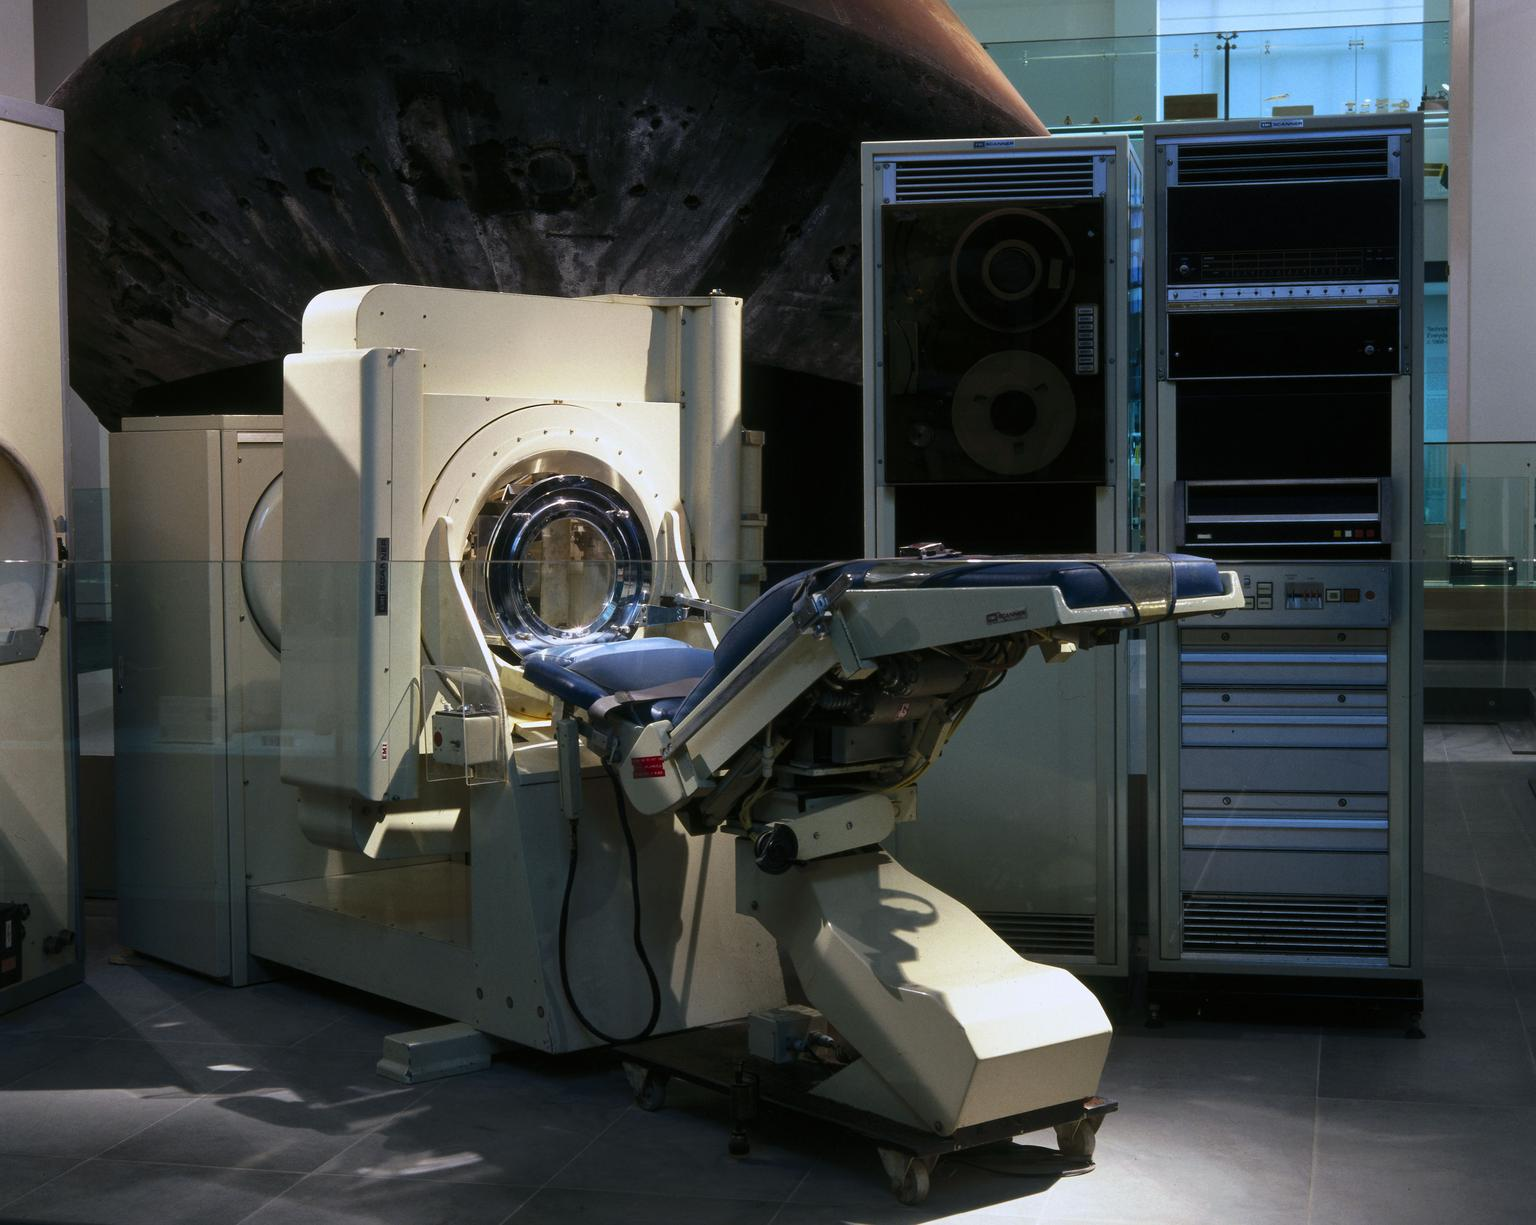
\includegraphics[width=0.4\textwidth, height=0.2\textwidth]{images/CT.jpg}
\caption{First EMI Scanner \cite{emict}}\label{fig:CT1010}
\end{figure}

\vfill{\null}

\section{Theory} \label{sec:theory}
\subsection{X-Ray Attenuation}
In X-ray tomography, images are modelled as attenuation coefficient distributions which is a measure of how much X-ray beams are attenuated when they propagate through an object. This problem can be modeled as in Eqn. \ref{eq:radon3d} for an arbitrary object.
\begin{equation} 
	I_{measured} = I_0 e^{-\iiint\limits_{object}\mu(x,y,z)dxdydz}
	\label{eq:radon3d}
\end{equation}
When the object to be imaged is two-dimensional or can be reduced to a two-dimensional slice, Eqn \ref{eq:radon3d} reduces to Eqn \ref{eq:radon2d}:
\begin{equation}
	I_{measured} = I_0 e^{-\iint\limits_{slice}\mu(x,y)dxdy}
	\label{eq:radon2d}
\end{equation}
\subsection{Radon Transform}
Radon Transform computes the line integrals along the objects to obtain projections along an arbitrary angle $\theta$ for an arbitrary beam t, using the formula given in Eqn. \ref{eq:radongeneral}.
\begin{equation}
	p_{\theta}(t) = \iint\limits_{-\infty}^{\ \ \ \infty}\mu(x,y)\delta(xcos(\theta)+ysin(\theta)-t)dxdy
	\label{eq:radongeneral}
\end{equation}
This equation models the X-ray beams as parallel lines through the object. In a more practical scenario, the X-ray source is modelled as a point source and beams are projected from source to the object in fan beam shape, due to the equiangular spaced discrete detector locations. This modelling can be achieved by introducing geometric transformation between projection variables. 

\begin{figure}[h]
\centering
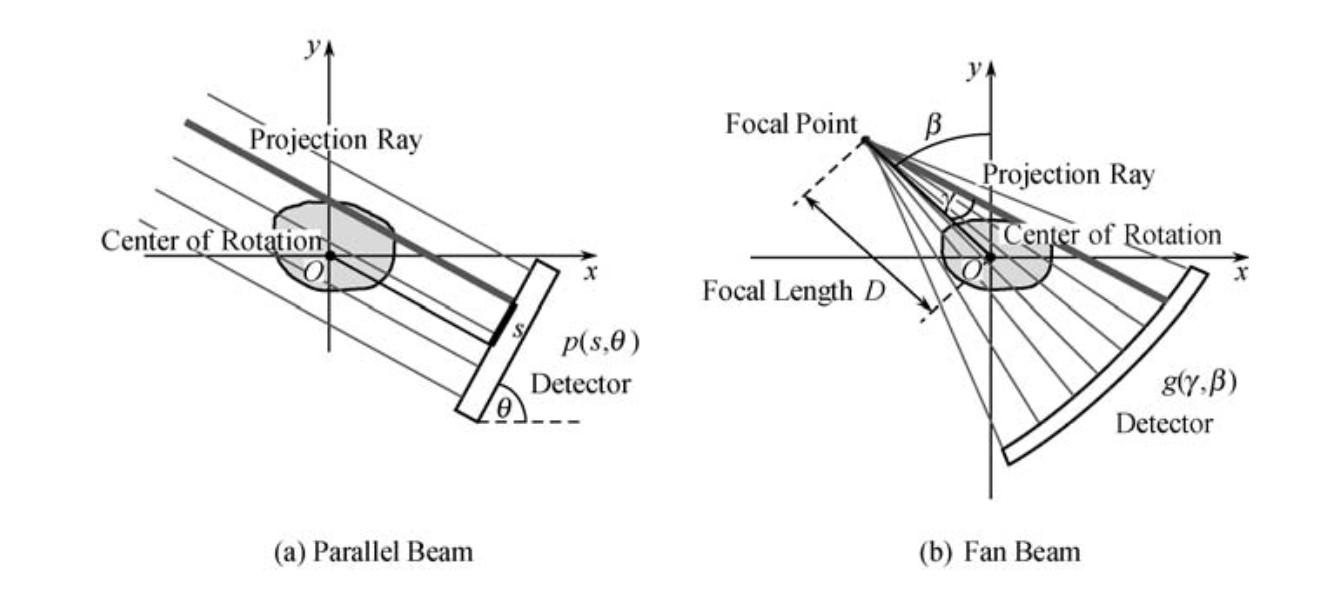
\includegraphics[width=0.3\textwidth]{images/PvsB.jpg}
\caption{Parallel Beams and Fan Beams \cite{zeng2017image}}\label{fig:PvsB}
\end{figure}

In Figure \ref{fig:PvsB}b, the projection angle with respect to center of rotation is defined as $\beta$ and the deviation from the center beam that is parallel to the $\beta$ beam is defined as $\gamma$ angles. In addition, the source to origin distance is labelled as $D$, resulting in source to detector distance of $2D$. 

With source to detector distance redefined as D and the remaining quantities defined as above, one could transform the equation in \ref{eq:radongeneral} to \ref{eq:transformedgeneral} using Eqn. \ref{eq:trans1} and \ref{eq:trans2}.
\begin{align}
	t &= D \cdot sin(\gamma) \label{eq:trans1} \\
	\theta &= \beta + \gamma \label{eq:trans2} \\
	p_{\beta}(\gamma) &= \iint\limits_{-\infty}^{\ \ \ \infty}\mu(x,y)\delta(xcos(\theta)+ysin(\theta) \label{eq:transformedgeneral} \\&-Dsin(\gamma))d\gamma d\beta \nonumber 
\end{align}

\subsection{Algebraic Reconstruction Technique}
The idea of converting the tomography problem to a linear system of equations and solving it iteratively originates from the technique which was first introduced by Gordon \textit{et al.} in \cite{gordon1970algebraic} for solving the problem of three-dimensional reconstruction from projections in electron microscopy and radiology. The method utilizes the Kaczmarz algorithm described in \cite*{kaczmarz1993approximate} as follows:

\begin{figure}[h]
\centering
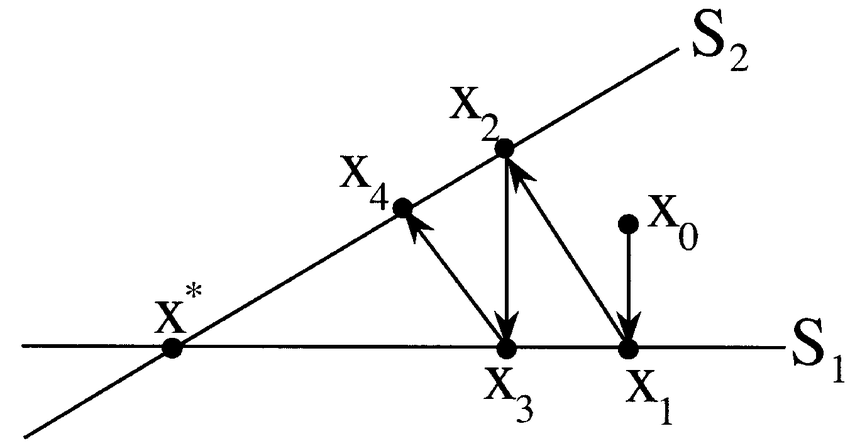
\includegraphics[width=0.3\textwidth]{images/Graphical-representation-of-the-Kaczmarzs-algorithm.png}
\caption{Kaczmarz Algorithm for solving linear systems of equations}\label{fig:kaczmarz}
\end{figure}

\begin{enumerate}
	\item Start with an initial random guess in the hyperspace of problem dimensions. 
	\item Project the solution vector onto the hyperplanes described by the rays whose parameters are determined by the line integrals taken along the corresponding ray. 
	\item Repeat the procedure until the termination condition is satisfied. This can be chosen as an error rate or number of iterations.  
\end{enumerate}

These steps can be summarized in the following update equation: 

\begin{equation}
	f^{(k+1)} = f^{(k)} - \alpha\frac{(f^Tw_j - p_j)}{||w||} 
\end{equation}

where f is the flattened image, $\alpha$ is the relaxation parameter, $w_j$ is the weights of the hyperplane defined by the $j_{th}$ ray and $p_j$ is the projection value of the corresponding ray. 
\\
\\
However, images reconstructed with this procedure exhibit a very noisy salt and pepper characteristic. To decrease the effect of this behavior without the changing the algorithm, one can optimize the order of selection of rays so that the projections hyperplanes are far from each other. This resulting in better quality pixel updates hence improves the convergence of the algorithm. This approach is utilized in the ART algorithm by default, by selecting hyperplanes that are separated by $\frac{FOV}{2}$ consecutively.

\subsection{Sequential Iterative Reconstruction Technique}

It is known that there is no single point intersections in the ART hyperplanes when the projections are corrupted by Poisson noise \cite*{dong2020accelerated}.  
In 1970, Gilbert \textit{et al.} in \cite*{gilbert1972iterative} proposed SIRT algorithm to overcome this effect by applying the computed pixel updates simultaneously, rather than equation by equation. 

In SIRT, the system $Ax=b$ where A is the projection matrix, is solved by minimizing the $\mathcal{L_2}$ norm cost function $$J = ||Ax-b||_2^2$$
Using gradient descent, the update formula becomes:
\begin{equation}
	f^{(k+1)} = f^{(k)} - \alpha A^T(Ax^{(k)}-b)
\end{equation}

In this equation, $A^T$ represents the back projection operator, since it is the adjoint operator of A. The reconstruction is performed by backprojecting the error to image space and updating the estimate by taking the difference of the error and the current guess hoping that error is going to be zeroed out, and the updates are going to stop. 
The authors of \cite*{dong2020accelerated} states that for $0<\alpha<\frac{2}{||A^TA||}$, the convergence of the algorithm is guaranteed. 

\subsection{Simultaneous Algebraic Reconstruction Technique}

Although SIRT exhibits a good performance when it is compared to ART, it requires much higher iterations to converge. Andersen \& Kak proposes a new method to estimate the overall image in fewer iterations by introducing a new pixel basis to the forward problem in \cite*{andersen1984sart}. The algorithm composes of the following steps:
\begin{enumerate}
	\item A circular reconstruction region inside the image is determined. 
	\item The crossing segment of the rays with reconstruction region is divided into $M$ equidistant points.
	\item The value of the continuous distribution of the image $\hat{f}$ is calculated by using the square-pyramid shaped bilinear elements with a support of 4 pixels.
	\item The projections are found as the integrations of the image estimates along that line. 
\end{enumerate}

\newpage

\section{Implementation} \label{sec:implementation}

In this section, the computer implementation of the scientific background explained in Section \nameref{sec:theory} is going to be described.

\subsection{Projection}
\begin{algorithm}[h]
\caption{Projection algorithm}
\begin{algorithmic}
\Procedure{PROJECTIONS}{$I,N_D, L_D, L_{SD}$} 
   \For{Projection angle $\beta$}
		 \For{Fan beam angle $\gamma$}
		\State Calculate x intersection
		\State Calculate y intersection
		\State Sort \Comment{Regular grid}
		\State Find distance between intersections \Comment{weights}
		\State Find the corresponding pixels
		\State Calculate projection \Comment{$weights \cdot I(pixels)$}
		\State Store in projection matrix
	  \EndFor
   \EndFor
   \State \textbf{return Projection matrix}
\EndProcedure
\label{alg:projection}
\end{algorithmic}
\end{algorithm}

\subsection{Reconstruction}

\begin{algorithm}[h]
	\caption{ART Algorithm}
	\begin{algorithmic}
		\Procedure{ART}{$PROJECTIONS,N_D, L_D, L_{SD}$} 
		\State Get the angle step size from Projections. 
		\State Get the number of the beams from Projections. 
		\State Set initial random guess $f^{(0)}$
		   \For{Projection angle $\beta$}
				 \For{Fan beam angle $\gamma$}\\
				\Comment{$Line = F(x,y,\beta,\gamma)$}
				\State Iteratively project the current solution on one of the hyperplanes defined by the ray equations.
				\State If Classical ART is utilized, the nonzero weights are replaced with ones. 
				\State Check the convergence to continue optimization.
			  \EndFor
		   \EndFor
		   \State Reshape the solution vector to image. 
		   \State \textbf{return IMAGE}
		\EndProcedure
	\label{alg:ART}
	\end{algorithmic}
\end{algorithm}

\begin{algorithm}[h]
	\caption{SIRT Algorithm}
	\begin{algorithmic}
		\Procedure{ART}{$PROJECTIONS,N_D, L_D, L_{SD}$} 
		\State Allocate projection matrix in sparse form.
		\State Get the angle step size from Projections. 
		\State Get the number of the beams from Projections. 
		\State Set initial random guess $f^{(0)}$
		   \For{Projection angle $\beta$}
				\For{Fan beam angle $\gamma$}
				\State Determine the weights corresponding to the current beam and the corresponding pixels.
				\State Place the weight vector into the matrix.
			  \EndFor
		   \EndFor
		   \For{iteration $n$}
				\State $f^{(k+1)} = f^{(k)} - \alpha A^T(Ax^{(k)}-b)$
		   \EndFor
		   \State Reshape the solution vector $f$ to image. 
		   \State \textbf{return IMAGE}
		\EndProcedure
	\label{alg:SIRT}
	\end{algorithmic}
\end{algorithm}

\begin{algorithm}[h]
	\caption{SART Algorithm}
	\begin{algorithmic}
		\Procedure{ART}{$PROJECTIONS,N_D, L_D, L_{SD}$} 
		\State Allocate projection matrix in sparse form.
		\State Get the angle step size from Projections. 
		\State Get the number of the beams from Projections. 
		\State Set initial random guess $f^{(0)}$
		   \For{Projection angle $\beta$}
				\For{Fan beam angle $\gamma$}
				\State Segment the line into $M$ equidistant vectors. 
				\State Find the distance $\Delta s$ between the consecutive points.
				\For{each pixel in the image}
					\State{Calculate the contribution $d_{ijm}$ to the $m^{th}$ point on the segment in terms of bilinear interpolation weights}
					\State {$a_{ij} = \sum d_{ijm}\Delta s$}
				\EndFor 
			  \EndFor
		   \EndFor
		   \For{iteration $n$}
				\State $f^{(k+1)} = f^{(k)} - \alpha A^T(Ax^{(k)}-b)$
		   \EndFor
		   \State Reshape the solution vector $f$ to image. 
		   \State \textbf{return IMAGE}
		\EndProcedure
	\label{alg:SART}
	\end{algorithmic}
\end{algorithm}

\newpage

The developed application implements the above algorithms in order to project and reconstruct the image. All components of the software and the Graphical User Interface is implemented in MATLAB(The MathWorks\textsuperscript{\textregistered}, Inc., Natick, Massachusetts, United States.) The guide to how to use the graphical user interface can be achieved in the README section of the following repository: \href{https://github.com/kutay-ugurlu/Fan-Beam-CT-ART-Simulation}{github.com/kutay-ugurlu/Fan-Beam-CT-ART-Simulation}.

\subsection{Early Stopping}
Since these algorithms use heuristic approaches or local optimizers, error metrics can diverge in some situations. To overcome this problem, an early stopping script is developed. This program keeps track of the current cumulated error vector that contains error metrics for previous iterations and takes an input called \textbf{patience}, which describes the number of iterations to wait for the algorithm to reduce the error in the next iteration. When this patience limit is achieved, algorithm outputs the reconstruction having the minimum relative error defined in Eqn. \ref{eqn:relativeerror}, where $\hat{x}$ represents the reconstructed image and $x$ represents the ground truth.  

\begin{equation}
	Relative Error = \frac{||\hat{x} - x||}{||x||} \label{eqn:relativeerror}
\end{equation}

\section{Results}\label{sec:results}

The experiments comparing the performances of the aforesaid algorithms are conducted using the following set of parameters: 

\begin{multicols}{2}
    \begin{itemize}
        \item $N_{iter}$ = 200
        \item $L_{detector}$ = 200
        \item $N_{detectors}$ = 100
        \item Source-Detector\newline distance = 200
        \item Projection angle \newline step size = $2^\circ$
        \item Relaxation $\alpha$ = 0.2
        \item Patience: 50 iterations
    \end{itemize}
    \end{multicols}

For phantom Lena, the original phantom is cropped to have 80 by 80 image. Considering that the number of pixels is increased by 2.56, number of rays in this case is increased to 200 to compensate for the increased image size. 

\begin{figure}[h]
	\centering
	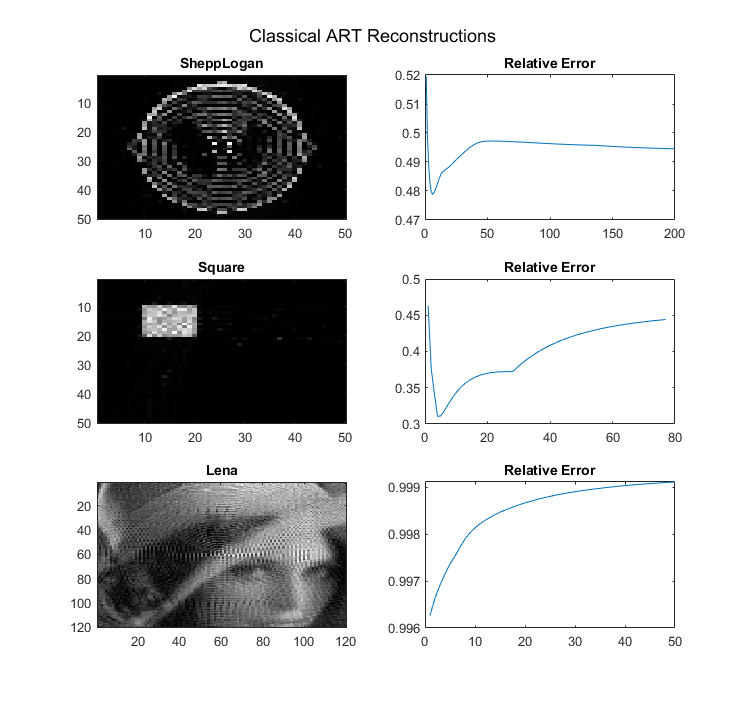
\includegraphics[width=0.4\textwidth, height=0.5\textwidth]{images/classical_art.png}
	\caption{Classical ART Reconstructions}\label{fig:cart}
\end{figure}
\begin{figure}[h]
	\centering
	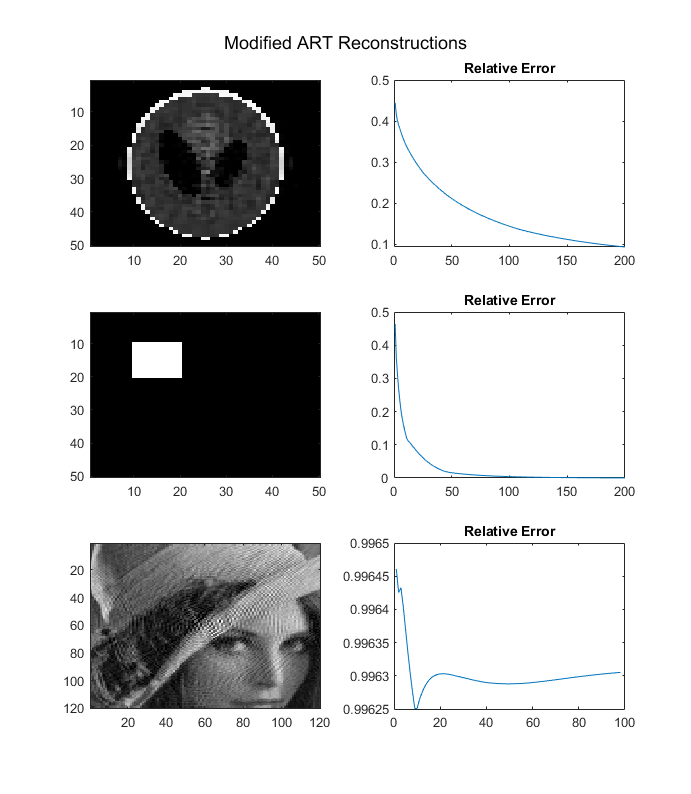
\includegraphics[width=0.4\textwidth, height=0.5\textwidth]{images/modifiedart.png}
	\caption{Modified ART Reconstructions}\label{fig:mart}
\end{figure}
\newpage
\begin{figure}[h]
	\centering
	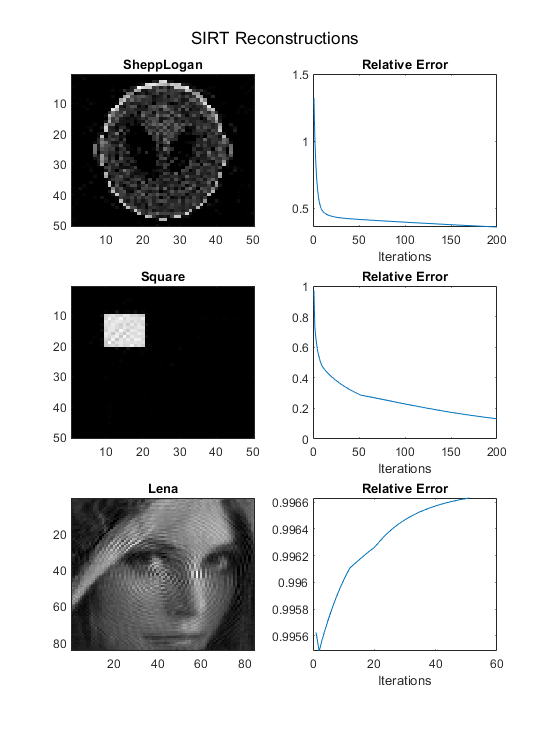
\includegraphics[width=0.4\textwidth, height=0.5\textwidth]{images/sirt.png}
	\caption{SIRT Reconstructions}\label{fig:sirt}
\end{figure}
\begin{figure}[h]
	\centering
	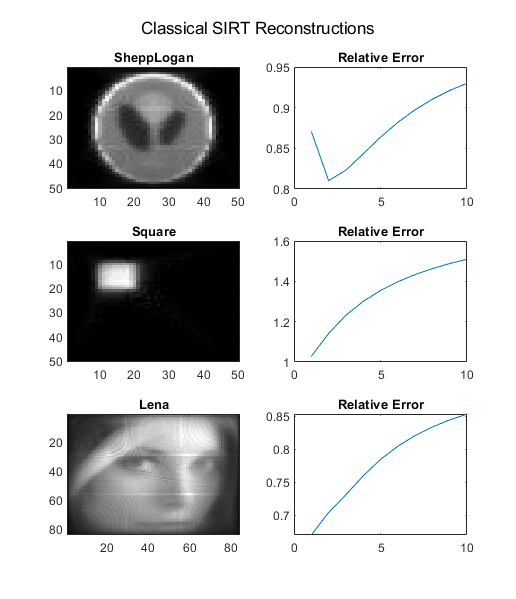
\includegraphics[width=0.4\textwidth, height=0.5\textwidth]{images/sart.png}
	\caption{SART Reconstructions}\label{fig:sart}
\end{figure}

\begin{table}[h]
	\centering
	\begin{tabular}{|c|c|c|c|c|}
		\hline 
		\diagbox{Phantom}{Algorithm} & ART & {Modified \newline ART} & SIRT & SART \\ 
		\hline 
		SheppLogan 	& 0.62 & 0.93 & 0.70 & 0.58 \\ 
		Square 		& 0.87 	& 1 & 0.99 & 0.72 \\ 
		Lena 		& 0 	& 0 & 0 & 0.42 \\ 
		\hline 
		\end{tabular}
	\caption{\label{tab:ssim}SSIM Index \cite*{wang2004image} for different reconstruction algorithms}
\end{table}

\newpage
\section{Discussion} \label{sec:discuss}

Figures \Cref*{fig:cart,fig:mart,fig:sirt,fig:sart} shows the reconstruction error in each iteration in the relative error metric defined by Eqn. \ref*{eqn:relativeerror}. In addition, the Structural Similarity(SSIM) \cite*{wang2004image} metric is utilized to perform a quantitative comparison between the reconstructed and ground-truth images.
\\
\\
\subsection{Classical and Modified ART}
It is known that classical ART implementation introduces salt and pepper patterned noise to the reconstruction images. In Figure \ref*{fig:cart} one can observe the high frequency noise clearly in SheppLogan and Square phantoms. Along with that, it can be observed that the relative error decreases in the first few iterations however it starts to increase afterwards. Furthermore, it is also obvious from the number of iterations (with 50 patience iterations) that the reconstructions diverges from the original result. This may be attributed to the fact that binary weighting strategy of classical ART algorithm constantly introduces noise due to the lack of quantification of contribution from different pixels. When we look at the Modified ART algorithm's results, on the other hand, we observe that algorithm has run for 200 iterations and exhibited a constant decreased in the error metric, resulting in a relative error around 0.05 for the first two phantoms. However, for higher dimensional solution spaces such as phantom Lena, this strategy does not work as good as it is in the remaining ones. Although the error minimization shows a steady decrease, the relative improvement with respect to the first iteration is remarkably low, being around 1\%. Nevertheless, the performance of the reconstruction is qualitatively moderate to human eye.  
\\
\\
\subsection{ART and SIRT}
It is observed that, for same number of iterations, the final error metric SIRT can achieve is higher than that of ART, \textit{i.e.} SIRT requires more iterations to converge where modified ART does, hence it verifies the fact stated in \cite*{dong2020accelerated} that SIRT may need approximately 200 hundred iterations to converge.  On the other hand, SIRT updates seems to provide better updates in the earlier iterations than ART. This is because it utilizes the all equations to at once to calculate the update on an image. However, it comes with the trade off that it has less sharp images than ART. 
\\
\\
\subsection{SART and SIRT}
SART algorithm treats the digital image as a continuous distribution of the image and projections as discrete ray sums of bilinear-interpolated estimates of image samples on the rays \cite*{andersen1984sart}. In other words, it transforms the basis from traditional pixel basis to bilinear element basis. Therefore, we observe a low-pass effect in the reconstructed images, since the algorithm aims to reconstruct a smooth distribution. This explains why the reconstructed phantoms are blurred in all cases. Overall, it seems to approximate the image visually well and can be utilized in cases where the projection data is limited and details in the image are not a concern.
\\
\\
\subsection{Lena phantom}
It is observed that reconstructions of phantom Lena has poor performance in terms of SSIM Index in Table \ref*{tab:ssim}. However, for modified ART and SIRT reconstructions, the qualitative visual performance of the reconstructions are satisfactory. On the contrary, the blurred SART reconstruction has a remarkably higher SSIM Index. This may arise from the fact that the predefined error metrics to decide where to stop in the optimization process may not be optimal, but instead suboptimal. In other words, $\mathcal{L_2}$ norm utilizing relative error metrics may not be the best option to evaluate the performance of the reconstruction. This becomes more clear when we compare the Relative Error and SSIM Index of the SIRT and SART reconstructions. Although there is 13\% difference in the relative metric, the structural similarity difference is about half a range. All in all, a visual (or qualitative) comparison should accompany the numerical metrics to achieve the best reconstructions. 
\\
\\
\subsection{Conclusion and Future work}
This project report theoretically explains and empirically validates the differences between the reconstruction of images via different algorithms. It was observed that for different situations, such as low number of projections and different objectives like obtaining sharp reconstructions, one can utilize different algorithms. Although main differences are stated utilizing the reconstruction of three phantoms, hyperparameters of the algorithms, such as choice of relaxation parameter, patience iterations was empirically found and utilized for single cases. The methods to choose these parameters may also be investigated to have better performance. Furthermore, a couple well known techniques such as early stopping and ray selection optimization is utilized to achieve the best performance. Some further modification can be investigated to make these methods more robust to projection and image sizes. 
\newpage
\printbibliography
\end{document}
